%%
%% EASE 2026 Industry Papers — Short Paper (4 pages + 1 page references)
%% Rewritten from CAIS 2026 PR #14 (v2): feedback loop framing, honest metrics
%%
\documentclass[sigconf]{acmart}

%% Rights management information
\setcopyright{acmlicensed}
\copyrightyear{2026}
\acmYear{2026}
\acmDOI{XXXXXXX.XXXXXXX}

%% Conference information
\acmConference[EASE '26]{International Conference on Evaluation and Assessment in Software Engineering}{June 9--12, 2026}{Glasgow, United Kingdom}
\acmBooktitle{Proceedings of the International Conference on Evaluation and Assessment in Software Engineering (EASE '26), June 9--12, 2026, Glasgow, United Kingdom}
\acmISBN{978-1-4503-XXXX-X/26/06}

%% Packages
\usepackage{booktabs}
\usepackage{amsmath}
\usepackage{multirow}
\usepackage{tikz}
\usetikzlibrary{shapes.geometric, calc}

%%
%% Document starts
%%
\begin{document}

%%
%% Title
%%
\title{CanItShip: Closing the Feedback Loop on Agent Tooling via Trajectory Analysis and Agentic DevX Metrics}

%%
%% Authors
%%
\author{Evgenii Kniazev}
\affiliation{%
  \institution{Databricks}
}
\email{evgenii.kniazev@databricks.com}

\author{Arseny Kravchenko}
\affiliation{%
  \institution{Databricks}
}
\email{arseny.kravchenko@databricks.com}

\author{Igor Rekun}
\affiliation{%
  \institution{Databricks}
}
\email{igor.rekun@databricks.com}

\author{Fabian Jakobs}
\affiliation{%
  \institution{Databricks}
}
\email{fabian.jakobs@databricks.com}

%%
%% Abstract
%%
\begin{abstract}
When AI agents fail to build production applications, should we improve the agent or its environment? Recent work suggests that environment quality (templates, tools, guidance) matters more than model selection~\cite{kniazev2025appbuild}. We present a feedback loop for iterative tooling improvement: (1)~an \emph{installable domain knowledge} architecture packages expertise as agent-consumable artifacts; (2)~agents use this package to generate applications, producing execution trajectories; (3)~an \emph{agentic trajectory analyzer} processes these trajectories to identify friction and recommend fixes to the package; (4)~\emph{Agentic DevX metrics} serve as the final quality gate, measuring whether generated applications can be operated by other agents. This approach is designed to generalize across domains; we validate it on Databricks data applications across multiple agent backends (Claude Code and Opencode). On 50~applications, we achieve 90\% one-shot build success at \$2.33/app. The trajectory analyzer identified concrete improvements (batch operations, clearer tool descriptions, missing examples) that we implemented, demonstrating the feedback loop mechanism through case studies. The architecture is designed for automatic optimization: the analyzer's recommendations target tool descriptions, prompts, and examples, artifacts amenable to techniques like GEPA or DSPy-style prompt tuning, potentially closing the loop without human intervention.
\end{abstract}

%%
%% CCS Concepts
%%
\begin{CCSXML}
<ccs2012>
   <concept>
       <concept_id>10011007.10011006.10011008.10011009.10011015</concept_id>
       <concept_desc>Software and its engineering~Software testing and debugging</concept_desc>
       <concept_significance>500</concept_significance>
   </concept>
   <concept>
       <concept_id>10011007.10011074.10011099.10011102.10011103</concept_id>
       <concept_desc>Software and its engineering~Software development process management</concept_desc>
       <concept_significance>300</concept_significance>
   </concept>
</ccs2012>
\end{CCSXML}

\ccsdesc[500]{Software and its engineering~Software testing and debugging}
\ccsdesc[300]{Software and its engineering~Software development process management}

%%
%% Keywords
%%
\keywords{CanItShip, agent-agnostic tooling, agentic code generation, trajectory analysis, developer experience metrics, feedback loop}

\maketitle

%% ============================================================
%% 1. INTRODUCTION
%% ============================================================
\section{Introduction}
\label{sec:intro}

AI agents can generate functional software, but they lack domain-specific knowledge required for production applications. The conventional response is building specialized agents. We take a different approach: improve what agents have access to.

This approach is motivated by recent findings~\cite{kniazev2025appbuild}: when comparing agent performance across environments while holding the model constant, environment quality (templates, tools, guidance) had larger effects than model upgrades. An agent with excellent tooling outperforms a better model with poor tooling.

Accepting that tooling matters raises a question: how do we improve it systematically? Manual inspection doesn't scale. End-state metrics (build pass/fail) don't reveal causes. We need a feedback loop that: (1)~captures how agents actually use tooling; (2)~identifies friction points and root causes; (3)~produces actionable recommendations; (4)~verifies improvements against agent-centric criteria.

We instantiate each component:

\begin{enumerate}
    \item \textbf{Installable Domain Knowledge} (Section~\ref{sec:domain-knowledge}). An architecture for packaging domain expertise as agent-consumable artifacts, exposing tools via CLI commands compatible with emerging skill-based standards.

    \item \textbf{Agentic Trajectory Analyzer} (Section~\ref{sec:trajectory}). A two-phase system: parallel friction extraction with a fast model followed by agentic synthesis with a reasoning model that has source code access.

    \item \textbf{CanItShip: Agentic DevX Metrics} (Section~\ref{sec:devx}). The final quality gate: all nine metrics are evaluated by an evaluator agent across three independent trials, measuring whether another agent, not a human, can reliably operate generated applications.
\end{enumerate}

\textbf{Validation.} We validate across Claude Code (primary) and Opencode on Databricks data applications. On 50~applications: 90\% build success, 90\% database connectivity, \$2.33/app average. The trajectory analyzer identified improvements that we implemented and verified through multiple iterations.

%% ============================================================
%% 2. INSTALLABLE DOMAIN KNOWLEDGE
%% ============================================================
\section{Installable Domain Knowledge}
\label{sec:domain-knowledge}

Developers already use capable agents (Claude Code, Opencode). Rather than asking them to adopt yet another tool, we bring domain knowledge to the agents they already use. A user installs our package into their existing environment; the agent gains domain expertise without workflow changes.

The package has three components: context layers that inject domain knowledge progressively, tools exposed via CLI, and a state machine that enforces validation before deployment.

\textbf{Context layers.} Agents have limited context windows. Dumping all domain knowledge upfront wastes tokens and can confuse the model. Instead, we inject context progressively; each layer activates when relevant (Table~\ref{tab:context-layers}).

\begin{table}[h]
\caption{Context layer injection strategy.}
\label{tab:context-layers}
\centering
\small
\begin{tabular}{llp{3.2cm}}
\toprule
\textbf{Layer} & \textbf{Content} & \textbf{When Injected} \\
\midrule
Tools & Tool names/descriptions & Always (protocol-level) \\
Workflow & Patterns, CLI usage & On first discovery call \\
Target & App vs job constraints & When target type detected \\
Template & SDK patterns, examples & After scaffolding \\
\bottomrule
\end{tabular}
\end{table}

\textbf{CLI tools.} We expose domain functionality through CLI commands, a pattern that Cloudflare~\cite{cloudflare2024codemode} and Anthropic~\cite{anthropic2024tools} found effective, reporting that LLMs perform better writing code to call CLI tools than invoking tools directly. Lifecycle commands (\texttt{scaffold}, \texttt{validate}, \texttt{deploy}) and data exploration commands (schema discovery, batch queries) provide the domain-specific capabilities on top of standard workspace tools.

\textbf{State machine.} Applications cannot deploy unless they pass validation after their most recent modification: \texttt{Scaffolded $\to$ Modified $\to$ Validated(checksum) $\to$ Deployed}. Any change after validation requires re-validation, preventing untested code deployment, a common failure mode when agents skip validation.

\textbf{Agent compatibility.} To validate agent-agnosticism, we tested the package across Claude Code (automated, primary) and Opencode with open-source models. The key requirement is function calling capability; any agent that can invoke CLI tools works with our package.

%% ============================================================
%% 3. AGENTIC TRAJECTORY ANALYZER
%% ============================================================
\section{Agentic Trajectory Analyzer}
\label{sec:trajectory}

The analyzer consumes execution trajectories and recommends package improvements. This closes the loop: agents struggle $\to$ we see it in trajectories $\to$ we fix the tooling $\to$ agents struggle less.

End-state metrics (build success, test pass) don't reveal whether failures stem from model limitations, tool problems, missing domain knowledge, or underspecified prompts. Trajectories (the sequence of reasoning, tool calls, and results) show where things went wrong. An agent retrying the same malformed SQL five times reveals a missing example. An agent calling N tools for N tables reveals a missing batch operation.

\textbf{Two-phase architecture.} We employ a map-reduce approach optimized for cost and quality. In the \emph{map phase}, each trajectory is processed independently by a fast model (Claude Haiku, ${\sim}\,$\$0.001 per trajectory), extracting errors, retries, confusion patterns, and inefficient tool usage. This runs in parallel. In the \emph{agentic synthesis phase}, aggregated patterns go to a reasoning model (Claude Opus) with read-only access to template source code, tool definitions, and prior analysis history, generating prioritized recommendations.

\textbf{Cost model.} For $N$ trajectories: map costs $N \times {\sim}\$0.001$ (fast model), synthesis costs ${\sim}\$0.5$--3 (reasoning model, bounded at 50~turns). For 50~apps, total analysis cost was under \$15.

\textbf{Human judgment on small N.} On small datasets, we found that the analyzer can overreact, encountering an issue once or twice and recommending building a helper utility without assessing maintenance cost~\cite{kravchenko2025mlsystem}. We recommend human review of recommendations when $N < 50$, treating the analyzer output as a prioritized error analysis rather than an implementation directive.

%% ============================================================
%% 4. AGENTIC DEVX METRICS
%% ============================================================
\section{Agentic DevX Metrics}
\label{sec:devx}

Agentic DevX is the final quality gate. After the package is improved and agents generate applications, we need to verify: can another agent actually operate this output?

Consider an agent that generates a working application. A human developer can run it: they'll figure out missing environment variables, install unlisted dependencies, work around unclear documentation. An agent \emph{can sometimes} do this too, but it's slow and inefficient, spending many turns on trial-and-error that explicit configuration would eliminate.

\textbf{Agentic evaluation protocol.} All nine metrics are evaluated by deploying an evaluator agent (Claude Haiku) that receives a prompt contract (Table~\ref{tab:prompts}) and emits a structured \texttt{STATUS: PASS|FAIL} verdict, parsed via regex with fallback inference. Each metric runs \emph{three independent trials}; a metric passes if all three trials succeed. Each trial records turns and token usage. A shell-script fallback exists for environments where the agent SDK is unavailable (e.g., root-only clusters).

\begin{table}[h]
\caption{Agentic evaluation prompt contracts.}
\label{tab:prompts}
\centering
\small
\begin{tabular}{lp{3.6cm}c}
\toprule
\textbf{Metric} & \textbf{Prompt Contract} & \textbf{Trials} \\
\midrule
L1: Build & Build app for production; run build scripts or import sanity & 3 \\
L2: Runtime & Start app, verify healthcheck responds on port & 3 \\
L3: Types & Run static/type checks (pyright, mypy, tsc) & 3 \\
L4: Tests & Run test suite; FAIL if no tests exist & 3 \\
\midrule
L5: DB Conn. & Connect to the database through the running app; verify query returns rows & 3 \\
L6: Data & Verify app returns real backend data, not mocked or hardcoded & 3 \\
L7: UI & Load UI on port; verify page renders without errors & 3 \\
D8: Runability & Install deps, start server, hit healthcheck endpoint & 3 \\
D9: Deploy & Build container, deploy, verify healthcheck returns 2xx & 3 \\
\bottomrule
\end{tabular}
\end{table}

\textbf{The CanItShip framework.} The nine metrics span three tiers: Core Functionality (L1--L4), Platform Integration (L5--L7), and Agentic DevX (D8--D9). The harness is platform-independent: prompt contracts reference generic concepts (database connectivity, healthcheck endpoints, container deployment) rather than platform-specific APIs.

%% --- Multi-agent comparison radar chart (9 axes) ---
\begin{figure}[t]
\centering
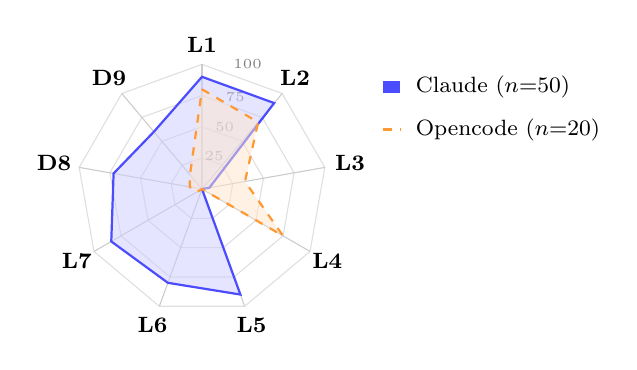
\begin{tikzpicture}[scale=0.72]
  % --- Radar grid (4 concentric 9-gons, 40° spacing) ---
  \foreach \l in {1,...,4} {
    \pgfmathsetmacro{\r}{\l/4*2.2}
    \draw[gray!25, thin]
      ({90}:\r) -- ({50}:\r) -- ({10}:\r) --
      ({-30}:\r) -- ({-70}:\r) -- ({-110}:\r) --
      ({-150}:\r) -- ({-190}:\r) -- ({-230}:\r) -- cycle;
  }
  % --- Axes ---
  \foreach \a in {90,50,10,-30,-70,-110,-150,-190,-230} {
    \draw[gray!40, thin] (0,0) -- (\a:2.2);
  }
  % --- Axis labels ---
  \node[font=\footnotesize\bfseries] at (90:2.55) {L1};
  \node[font=\footnotesize\bfseries] at (50:2.55) {L2};
  \node[font=\footnotesize\bfseries] at (10:2.65) {L3};
  \node[font=\footnotesize\bfseries] at (-30:2.55) {L4};
  \node[font=\footnotesize\bfseries] at (-70:2.55) {L5};
  \node[font=\footnotesize\bfseries] at (-110:2.55) {L6};
  \node[font=\footnotesize\bfseries] at (-150:2.55) {L7};
  \node[font=\footnotesize\bfseries] at (-190:2.65) {D8};
  \node[font=\footnotesize\bfseries] at (-230:2.55) {D9};
  % --- Scale labels (25%, 50%, 75%, 100%) ---
  \node[font=\tiny, gray] at (70:0.62) {25};
  \node[font=\tiny, gray] at (70:1.17) {50};
  \node[font=\tiny, gray] at (70:1.72) {75};
  \node[font=\tiny, gray] at (70:2.35) {100};
  % --- Claude Code (n=50): blue, solid ---
  % L1=90%, L2=90%, L3=6%, L4=0(n/a), L5=90%, L6=80%, L7=84%, D8=72%, D9=60%
  \fill[blue!20, opacity=0.5]
    (90:1.98) -- (50:1.98) -- (10:0.132) --
    (-30:0.0) -- (-70:1.98) -- (-110:1.76) --
    (-150:1.848) -- (-190:1.584) -- (-230:1.32) -- cycle;
  \draw[blue!70, thick]
    (90:1.98) -- (50:1.98) -- (10:0.132) --
    (-30:0.0) -- (-70:1.98) -- (-110:1.76) --
    (-150:1.848) -- (-190:1.584) -- (-230:1.32) -- cycle;
  % --- Opencode+Sonnet (n=20): orange, dashed ---
  % L1=80%, L2=70%, L3=35%, L4=75%, L5=0%, L6=0%, L7=5%, D8=10%, D9=15%
  \fill[orange!20, opacity=0.5]
    (90:1.76) -- (50:1.54) -- (10:0.77) --
    (-30:1.65) -- (-70:0.0) -- (-110:0.0) --
    (-150:0.11) -- (-190:0.22) -- (-230:0.33) -- cycle;
  \draw[orange!80, thick, dashed]
    (90:1.76) -- (50:1.54) -- (10:0.77) --
    (-30:1.65) -- (-70:0.0) -- (-110:0.0) --
    (-150:0.11) -- (-190:0.22) -- (-230:0.33) -- cycle;
  % --- Legend ---
  \fill[blue!70] (3.2,1.7) rectangle (3.5,1.9);
  \node[font=\footnotesize, anchor=west] at (3.6, 1.8) {Claude ($n{=}50$)};
  \draw[orange!80, thick, dashed] (3.2,1.05) -- (3.5,1.05);
  \node[font=\footnotesize, anchor=west] at (3.6, 1.05) {Opencode ($n{=}20$)};
\end{tikzpicture}
\caption{Multi-agent metric profiles (all 9 metrics). Claude Code (solid) achieves broad coverage but dips on L3 (type safety, 6\%) and L4 (tests, not yet evaluated). Opencode+Sonnet (dashed, $n{=}20$) shows moderate core metrics (L1=80\%, L4=75\%) and collapses on platform metrics (L5--L7), with D8/D9 provisional.}
\label{fig:radar}
\end{figure}

\textbf{Generation--evaluation isolation.} We observed agents reading evaluation scripts when both resided in the same workspace, producing code that passes checks rather than solving the underlying task. This is a form of reward hacking~\cite{amodei2016concrete}. We enforce container-level isolation via Dagger~\cite{dagger2024}: the generation Dockerfile copies only domain package code, explicitly excluding evaluation scripts. Each generation starts from a clean workspace. This mirrors training/test splits in ML; we recommend container-level isolation as a baseline requirement for agent evaluation.

%% ============================================================
%% 5. RESULTS
%% ============================================================
\section{Results}
\label{sec:results}

We evaluated on 50~Databricks applications spanning dashboards, analytics tools, and business intelligence interfaces. Each was generated from a natural language prompt using Claude Code with CLI-based tool orchestration in containerized execution.

\begin{table}[t]
\caption{Evaluation results ($n{=}50$ Databricks applications).}
\label{tab:results}
\centering
\small
\begin{tabular}{llc}
\toprule
\textbf{Tier} & \textbf{Metric} & \textbf{Result} \\
\midrule
\multirow{4}{*}{Core} & L1: Build Success & 45/50 (90\%) \\
 & L2: Runtime Success & 45/50 (90\%) \\
 & L3: Type Safety & 3/50 (6\%) \\
 & L4: Tests Pass & --$^{*}$ \\
\midrule
\multirow{3}{*}{Platform} & L5: DB Connectivity & 45/50 (90\%) \\
 & L6: Data Returned & 40/50 (80\%) \\
 & L7: UI Renders & 42/50 (84\%) \\
\midrule
\multirow{2}{*}{DevX} & D8: Runability & 36/50 (72\%) \\
 & D9: Deployability & 30/50 (60\%) \\
\midrule
\multirow{2}{*}{Efficiency} & Cost per App & \$2.33 \\
 & Lines of Code & 732 avg \\
\bottomrule
\multicolumn{3}{l}{\scriptsize $^{*}$L4 instrumented for Opencode (75\%) but not for the primary $n{=}50$ Claude evaluation.}
\end{tabular}
\end{table}

The 90\% build/runtime success indicates the core generation pipeline works. The drop from 90\% on single-trial metrics to 72\%/60\% on multi-trial D8/D9 quantifies the gap between ``code that works'' and ``code an agent can reliably operate'', the core motivation for Agentic DevX. 95\% Wilson confidence intervals for key metrics: L1/L2 [79\%, 96\%], D8 [58\%, 83\%], D9 [46\%, 73\%].

\textbf{Multi-agent comparison.} To validate agent-agnosticism, we ran the same CanItShip harness on 20~applications generated by Opencode with Sonnet (Table~\ref{tab:multiagent}). The pattern is clear: Opencode achieves 80\% build and 75\% test pass but collapses on platform metrics (L5--L7: 0\% DB connectivity, 0\% data returned). These applications compile but never connect to Databricks, returning mocked or empty data. This confirms that without installable domain knowledge, even a capable model produces structurally correct but domain-disconnected applications.

\begin{table}[h]
\caption{Multi-agent comparison: Claude Code ($n{=}50$) vs Opencode+Sonnet ($n{=}20$).}
\label{tab:multiagent}
\centering
\small
\begin{tabular}{lccc}
\toprule
\textbf{Metric} & \textbf{Claude Code} & \textbf{Opencode} & \textbf{$\Delta$} \\
\midrule
L1: Build & 90\% & 80\% & $-$10 \\
L2: Runtime & 90\% & 70\% & $-$20 \\
L3: Types & 6\% & 35\% & +29 \\
L4: Tests & --$^{*}$ & 75\% & -- \\
L5: DB Conn. & 90\% & 0\% & $-$90 \\
L6: Data & 80\% & 0\% & $-$80 \\
L7: UI & 84\% & 5\% & $-$79 \\
D8: Runability$^{\dagger}$ & 72\% & 10\% & $-$62 \\
D9: Deploy$^{\dagger}$ & 60\% & 15\% & $-$45 \\
\bottomrule
\multicolumn{4}{l}{\scriptsize $^{\dagger}$D8/D9 are provisional harness outputs for the Opencode evaluation.}
\end{tabular}
\end{table}

\textbf{Agentic metric variance.} The 3-trial protocol reveals significant non-determinism in agentic evaluation. Figure~\ref{fig:trials} shows both agents' metric profiles: Claude Code (a) achieves broad, stable coverage; Opencode (b) shows three independent trials with visible variance on D8 and D9. D8 trial-level pass rates range from 35\% to 50\% across trials, while D9 ranges from 30\% to 35\%. Per-app agreement: 50\% for D8 (10/20~apps consistent across all trials), 60\% for D9 (12/20~consistent). Mean trial-level D8: 41.7\% ($\sigma{=}7.6\%$); mean trial-level D9: 33.3\% ($\sigma{=}2.9\%$). Under the strict 3/3 pass criterion, only 2/20 apps pass D8 and 3/20 pass D9, demonstrating why multiple trials are essential for agentic evaluation.

%% --- Two-panel radar: Claude aggregate + Opencode 3-trial (9 axes) ---
\begin{figure}[t]
\centering
\begin{minipage}{0.48\columnwidth}
\centering
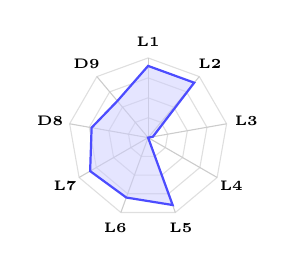
\begin{tikzpicture}[scale=0.46]
  % --- Radar grid (4 concentric 9-gons, 40° spacing) ---
  \foreach \l in {1,...,4} {
    \pgfmathsetmacro{\r}{\l/4*2.2}
    \draw[gray!25, thin]
      ({90}:\r) -- ({50}:\r) -- ({10}:\r) --
      ({-30}:\r) -- ({-70}:\r) -- ({-110}:\r) --
      ({-150}:\r) -- ({-190}:\r) -- ({-230}:\r) -- cycle;
  }
  % --- Axes ---
  \foreach \a in {90,50,10,-30,-70,-110,-150,-190,-230} {
    \draw[gray!40, thin] (0,0) -- (\a:2.2);
  }
  % --- Axis labels ---
  \node[font=\tiny\bfseries] at (90:2.65) {L1};
  \node[font=\tiny\bfseries] at (50:2.65) {L2};
  \node[font=\tiny\bfseries] at (10:2.75) {L3};
  \node[font=\tiny\bfseries] at (-30:2.65) {L4};
  \node[font=\tiny\bfseries] at (-70:2.65) {L5};
  \node[font=\tiny\bfseries] at (-110:2.65) {L6};
  \node[font=\tiny\bfseries] at (-150:2.65) {L7};
  \node[font=\tiny\bfseries] at (-190:2.75) {D8};
  \node[font=\tiny\bfseries] at (-230:2.65) {D9};
  % --- Claude Code aggregate (n=50): blue, solid ---
  % L1=90%, L2=90%, L3=6%, L4=0(n/a), L5=90%, L6=80%, L7=84%, D8=72%, D9=60%
  \fill[blue!20, opacity=0.5]
    (90:1.98) -- (50:1.98) -- (10:0.132) --
    (-30:0.0) -- (-70:1.98) -- (-110:1.76) --
    (-150:1.848) -- (-190:1.584) -- (-230:1.32) -- cycle;
  \draw[blue!70, thick]
    (90:1.98) -- (50:1.98) -- (10:0.132) --
    (-30:0.0) -- (-70:1.98) -- (-110:1.76) --
    (-150:1.848) -- (-190:1.584) -- (-230:1.32) -- cycle;
\end{tikzpicture}\\[1mm]
{\scriptsize (a) Claude Code ($n{=}50$, aggregate)}
\end{minipage}
\hfill
\begin{minipage}{0.48\columnwidth}
\centering
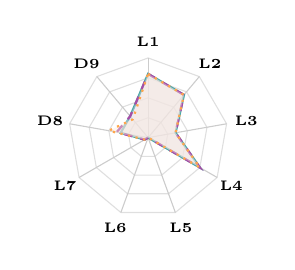
\begin{tikzpicture}[scale=0.46]
  % --- Radar grid (4 concentric 9-gons, 40° spacing) ---
  \foreach \l in {1,...,4} {
    \pgfmathsetmacro{\r}{\l/4*2.2}
    \draw[gray!25, thin]
      ({90}:\r) -- ({50}:\r) -- ({10}:\r) --
      ({-30}:\r) -- ({-70}:\r) -- ({-110}:\r) --
      ({-150}:\r) -- ({-190}:\r) -- ({-230}:\r) -- cycle;
  }
  % --- Axes ---
  \foreach \a in {90,50,10,-30,-70,-110,-150,-190,-230} {
    \draw[gray!40, thin] (0,0) -- (\a:2.2);
  }
  % --- Axis labels ---
  \node[font=\tiny\bfseries] at (90:2.65) {L1};
  \node[font=\tiny\bfseries] at (50:2.65) {L2};
  \node[font=\tiny\bfseries] at (10:2.75) {L3};
  \node[font=\tiny\bfseries] at (-30:2.65) {L4};
  \node[font=\tiny\bfseries] at (-70:2.65) {L5};
  \node[font=\tiny\bfseries] at (-110:2.65) {L6};
  \node[font=\tiny\bfseries] at (-150:2.65) {L7};
  \node[font=\tiny\bfseries] at (-190:2.75) {D8};
  \node[font=\tiny\bfseries] at (-230:2.65) {D9};
  % --- Trial 1: L1=80%,L2=70%,L3=35%,L4=75%,L5-L6=0%,L7=5%,D8=35%,D9=35% (solid teal) ---
  \fill[teal!15, opacity=0.4]
    (90:1.76) -- (50:1.54) -- (10:0.77) --
    (-30:1.65) -- (-70:0.0) -- (-110:0.0) --
    (-150:0.11) -- (-190:0.77) -- (-230:0.77) -- cycle;
  \draw[teal!70, thick]
    (90:1.76) -- (50:1.54) -- (10:0.77) --
    (-30:1.65) -- (-70:0.0) -- (-110:0.0) --
    (-150:0.11) -- (-190:0.77) -- (-230:0.77) -- cycle;
  % --- Trial 2: D8=40%,D9=35% (dashed violet) ---
  \fill[violet!15, opacity=0.4]
    (90:1.76) -- (50:1.54) -- (10:0.77) --
    (-30:1.65) -- (-70:0.0) -- (-110:0.0) --
    (-150:0.11) -- (-190:0.88) -- (-230:0.77) -- cycle;
  \draw[violet!70, thick, dashed]
    (90:1.76) -- (50:1.54) -- (10:0.77) --
    (-30:1.65) -- (-70:0.0) -- (-110:0.0) --
    (-150:0.11) -- (-190:0.88) -- (-230:0.77) -- cycle;
  % --- Trial 3: D8=50%,D9=30% (dotted orange) ---
  \fill[orange!15, opacity=0.4]
    (90:1.76) -- (50:1.54) -- (10:0.77) --
    (-30:1.65) -- (-70:0.0) -- (-110:0.0) --
    (-150:0.11) -- (-190:1.10) -- (-230:0.66) -- cycle;
  \draw[orange!70, thick, dotted]
    (90:1.76) -- (50:1.54) -- (10:0.77) --
    (-30:1.65) -- (-70:0.0) -- (-110:0.0) --
    (-150:0.11) -- (-190:1.10) -- (-230:0.66) -- cycle;
\end{tikzpicture}\\[1mm]
{\scriptsize (b) Opencode+Sonnet ($n{=}20$, 3 trials)}
\end{minipage}
\\[2mm]
% --- Shared legend ---
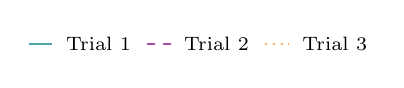
\begin{tikzpicture}
  \draw[teal!70, thick] (0,0) -- (0.3,0);
  \node[font=\scriptsize, anchor=west] at (0.35, 0) {Trial 1};
  \draw[violet!70, thick, dashed] (1.5,0) -- (1.8,0);
  \node[font=\scriptsize, anchor=west] at (1.85, 0) {Trial 2};
  \draw[orange!70, thick, dotted] (3.0,0) -- (3.3,0);
  \node[font=\scriptsize, anchor=west] at (3.35, 0) {Trial 3};
\end{tikzpicture}
\caption{Detailed metric profiles (all 9 metrics). (a)~Claude Code: broad coverage; L4 not yet evaluated. (b)~Opencode+Sonnet ($n{=}20$): three trial-level aggregates show moderate core metrics, platform metrics near 0\%, and visible D8/D9 variance across trials.}
\label{fig:trials}
\end{figure}

\textbf{Feedback loop mechanism: case studies.} The trajectory analyzer identified concrete friction points that we fixed in the domain package (Table~\ref{tab:improvements}). Agents calling schema discovery once per table (N calls for N tables) revealed a missing batch operation; we added it and observed agents using the batch call in subsequent generations. Repeated SQL syntax errors on \texttt{QUALIFY} and \texttt{PIVOT} clauses indicated missing dialect-specific examples; we added them to the guidance layer. A tool name mismatch caused agents to hallucinate tool calls; renaming for clarity eliminated the pattern. We demonstrate the mechanism produces actionable recommendations; quantifying cumulative improvement across iterations requires a longitudinal study. These fixes target tool descriptions, prompts, and examples---artifacts amenable to automatic optimization~\cite{gepa2025, khattab2023dspy}. The full trajectory analysis reports are available in the project repository.

\begin{table}[h]
\caption{Trajectory-identified improvements (implemented).}
\label{tab:improvements}
\centering
\small
\begin{tabular}{lp{1.8cm}p{2.4cm}}
\toprule
\textbf{Pattern Found} & \textbf{Root Cause} & \textbf{Fix Applied} \\
\midrule
N calls for N tables & Missing batch op & Added batch schema discovery \\
Repeated SQL errors & Missing examples & Added QUALIFY, PIVOT to guidance \\
Confusing tool name & Name mismatch & Renamed tool for clarity \\
Retries on errors & Unclear messages & Added contextual error params \\
6\% type safety & Missing null examples & Added null handling to templates \\
\bottomrule
\end{tabular}
\end{table}

%% ============================================================
%% 6. RELATED WORK
%% ============================================================
\section{Related Work}
\label{sec:related}

\textbf{Environment over model.} Recent work~\cite{kniazev2025appbuild} found that environment quality had larger effects than model upgrades when comparing agent performance. SWE-agent~\cite{yang2024swe} similarly demonstrated that agent-computer interfaces significantly affect performance. This motivates our focus on improving tooling rather than agents.

\textbf{Evaluation gap.} Existing benchmarks evaluate code correctness (HumanEval~\cite{chen2021evaluating}, SWE-bench~\cite{jimenez2024swe}), task completion (WebArena~\cite{zhou2024webarena}, GAIA~\cite{mialon2023gaia}), or SQL quality (BIRD~\cite{bird2023}, Spider~\cite{yu2018spider}). None ask whether generated code can be operated by other agents, a critical question for compound AI systems.

\textbf{Trajectory analysis.} Analyzing agent execution traces for debugging is established practice (SWE-agent~\cite{yang2024swe}, OpenHands~\cite{wang2024openhands}). Our contribution is making the synthesis phase itself agentic: an agent that explores source code to generate recommendations, rather than static aggregation.

\textbf{Agent evaluation harnesses.} Inspect AI~\cite{inspectai2024} and DeepEval~\cite{deepeval2024} provide evaluation infrastructure but focus on correctness rather than deployment readiness. AgentBench~\cite{agentbench2023} spans multiple environments but does not evaluate autonomous deployability. DORA metrics~\cite{forsgren2018accelerate} provide the industry standard for delivery performance; to our knowledge, no existing framework maps AI code generation evaluation to DORA.

%% ============================================================
%% 7. DISCUSSION
%% ============================================================
\section{Discussion}
\label{sec:discussion}

\textbf{Agent-agnostic vs agent-specific.} Our approach invests in tooling rather than agents: agents improve rapidly (model upgrades are free to adopters), while domain knowledge is slow to encode and hard to transfer. The tradeoff is control; agent-specific approaches can fine-tune behavior precisely, while we rely on the agent's ability to follow tool descriptions. In practice, this suffices for structured tasks but limits open-ended architectural reasoning.

\textbf{Toward automatic optimization.} Our loop is currently semi-automatic: the analyzer outputs recommendations, a human reviews them. Since recommendations target tool descriptions and prompts, techniques like GEPA~\cite{gepa2025} and DSPy~\cite{khattab2023dspy} could potentially close the loop without human intervention.

\textbf{Limitations.} \emph{External validity:} We validate on Databricks; the harness is platform-independent but domain packages require platform-specific implementation. \emph{Internal validity:} $n{=}50$ provides initial validation; scaling to 100+ across difficulty tiers is planned. \emph{Construct validity:} All metrics rely on evaluator agent judgment, introducing variance (Figure~\ref{fig:trials}). On small $N$, the trajectory analyzer can overreact to isolated failures; human review remains essential. The feedback loop is demonstrated qualitatively through case studies (Table~\ref{tab:improvements}); longitudinal quantification across multiple iterations with $n{=}100$+ is planned.

%% ============================================================
%% 8. CONCLUSION
%% ============================================================
\section{Conclusion}
\label{sec:conclusion}

We presented a feedback loop for iterative improvement of agent tooling: installable domain knowledge, an agentic trajectory analyzer, and Agentic DevX metrics. On 50~Databricks applications across multiple agent backends, we achieve 90\% build success at \$2.33/app. The trajectory analyzer identified concrete improvements that we implemented and verified. When agents fail, improve their environment rather than the agents themselves. The evaluation harness, trajectory analyzer, 50-prompt benchmark, and anonymized artifacts are released under the MIT license.

%%
%% Acknowledgments
%%
\begin{acks}
We thank the Databricks Apps team for infrastructure support and the internal hackathon participants whose prompts formed the basis of our benchmark.
\end{acks}

%%
%% Bibliography
%%
\bibliographystyle{ACM-Reference-Format}
\bibliography{references}

\end{document}
